One of the goals of this thesis is creating of a~simple application which demonstrates functionality of OptaPlanner tool
on Android system. Previous Chapter~\ref{PortingChapter} shows how to port the tool to the mobile platform. In this
chapter, OptaPlanner tool is used to creating the Vehicle Routing Problem application.

First Section~\ref{RequirementsApplicationSection} introduces application requirements. Application design is described
in the second Section~\ref{ApplicationDesignSection}. Implementation itself is divided into two parts. The first part
which is described in Section~\ref{ApplicationImplementationSection} present inner structure of the application and the
second part deals with graphical user interface and its layout.

\section{Requirements for Android application}\label{RequirementsApplicationSection}
This section deals with requirements for Android application. First part introduces features of the application and the
second part discusses support for different versions of the Android operating system.

\subsection{Application features}\label{FeaturesSection}
The following paragraphs describe essential requirements and features of created application. They focus on inner
structure, graphical user interface and the licence under which the application is written.

\paragraph{Vehicle Routing application}
Standard OptaPlanner distribution~\cite{OptaPlannerDistribution} contains demonstration examples. One of the examples is
Vehicle Routing application. It is often used for presentation of OptaPlanner and it is one of the real world examples
and thus it is also a~good choice for demonstration on Android. Created aplication should present the Vehicle Routing
Problem in a~similar way as the original OptaPlanner application.

\paragraph{Vehicle Routing model}
The source code of the original application already contains OptaPlanner Vehicle Routing Problem model which should be
included in this application. Furthermore, it contains some tools for importing specific \texttt{.vrp} files. The model
specifies classes which are required for OptaPlanner tool.

\paragraph{Graphical user interface}
Graphical user interface cannot be ported because application is written by Awt and Swing libraries which are not
included in Android API as described in Section~\ref{ComparsionSection}. Therefore, new application graphical user
interface should be created and adjusted to fulfill aspects of Android application development.

\paragraph{Application settings}
Application without any settings is too static and uninteresting for the users. Therefore, they should at least be able
to choose problem solving algorithm. Another option could be setting of calculation time limit. Thanks to that, process
can be terminated earlier.

\paragraph{File opening}
The original Vehicle Routing application contains \texttt{.vrp} example files which contains tasks of problems. These
files should be compatible with created application and some of them should be included. It should be possible to open
these files and display them in a~similar way as in the original application.

\paragraph{Solution displaying}
The application must be able to display unsolved solution on the application screen. Furthermore, it should be possible
to display new best solution everytime when it is found and at the end of the process, last best solution should remain
on the screen. The application should also be able to display actual statistic information about solved problem.

\paragraph{License}
The entire application should be distributed as an~open-source software and it should be written under Apache License
2.0. Source code must be publicly available on the Internet for guidance of other people in their own OptaPlanner
projects.

\subsection{Android devices support}
Before the development starts, it is good to clarify which version of Android will be supported by application. Every
version of Android comes with new API and new functionality. Biggest changes comes when the first number of version is
changed. Actual distributions of Android versions on devices can be seen in the last column of
Table~\ref{AndroidHistoryTable}.

Versions 2.x.x are on decline. Currently, the most used versions are with 4.x designation and distribution of the newest
5.x versions grows. Therefore, it is decided that application should support Android from version 4.0 (API 14). The
version decides which resource can be used for application design and development and how application should be tested.

\section{Application design}\label{ApplicationDesignSection}
One of the critical points of creating an~application is design. It can be divided into two parts. The first one is
design of an~innner structure and it is presented in Section~\ref{ApplicationFeatureSection}. The second one is design
of graphical user interface and application component layout which is described in Section~\ref{ScreenDesignSection}.

\subsection{Application features}\label{ApplicationFeatureSection}
In Section~\ref{FeaturesSection}, inner structure requirements of the application are described. According to them, the
application features design is written and introduced in following paragraphs.

\paragraph{Application settings}
Designed application supports several setting options. It is possible to select one of three algorithms: First fit
decreasing with Late acceptance, Branch and bound and Brute force. Simultaneously, it is required to select time limit
of calculation in seconds. Calculation stops after time limit is reached or it is possible to stop it earlier by stop
button. Furthermore, Vehicle Routing example can be chosen. Application contains list of these files and after user
selects one of them everything should be prepared to calculation start. The setting should be placed on the first screen
of the application.

\paragraph{VRP files}
Mentioned list of example files consists from files used in original OptaPlanner application. These files are named the
same way and user can compare results between both applications. Because default Android system does not contain file
browser and user probably does not have his own \texttt{.vrp} files, application does not support opening files from
device storage. List of files should be placed on the second screen of the application.

\paragraph{Porting of Vehicle Routing Problem model}
In Section~\ref{FeaturesSection}, it is described that original application already contains Vehicle Routing model for
OptaPlanner tool. These classes have to be embedded into application and they have to be used for calculation of the
problem. Furthermore, they should be used for displaying of current solution.

\paragraph{Problem solving}
Graphical user interface cannot wait until calculation is finished and therefore these two parts must be separated from
each other. While solving is in progress, user controls the application and also can use some of its parts. When screen
is turned or application is hidden in background, solving process has to be still active and not terminated.

\paragraph{Solution displaying}
New best solution should be displayed every time when it is found. For that purpose, application contains third screen
especially for displaying founded solution which should be similar to original application. Lines represents roads,
vehicles and depots have their own icons. Customers differs from the original for saving screen space. Intead of points
with numbers, customers should be represented as circles with inner number describing its demand. Time window circles
should be displayed in a~similar way as the original but not separated from customer.

\paragraph{Solution data}
Every solution has data which cannot be displayed graphically or they are too important and have to be be displayed
separately. Hence, it is designed that score of solution and actual load of vehicles should be drawn on side menu which
is described in Section~\ref{ScreenDesignSection}.

\begin{figure}[h!]
    \centering
    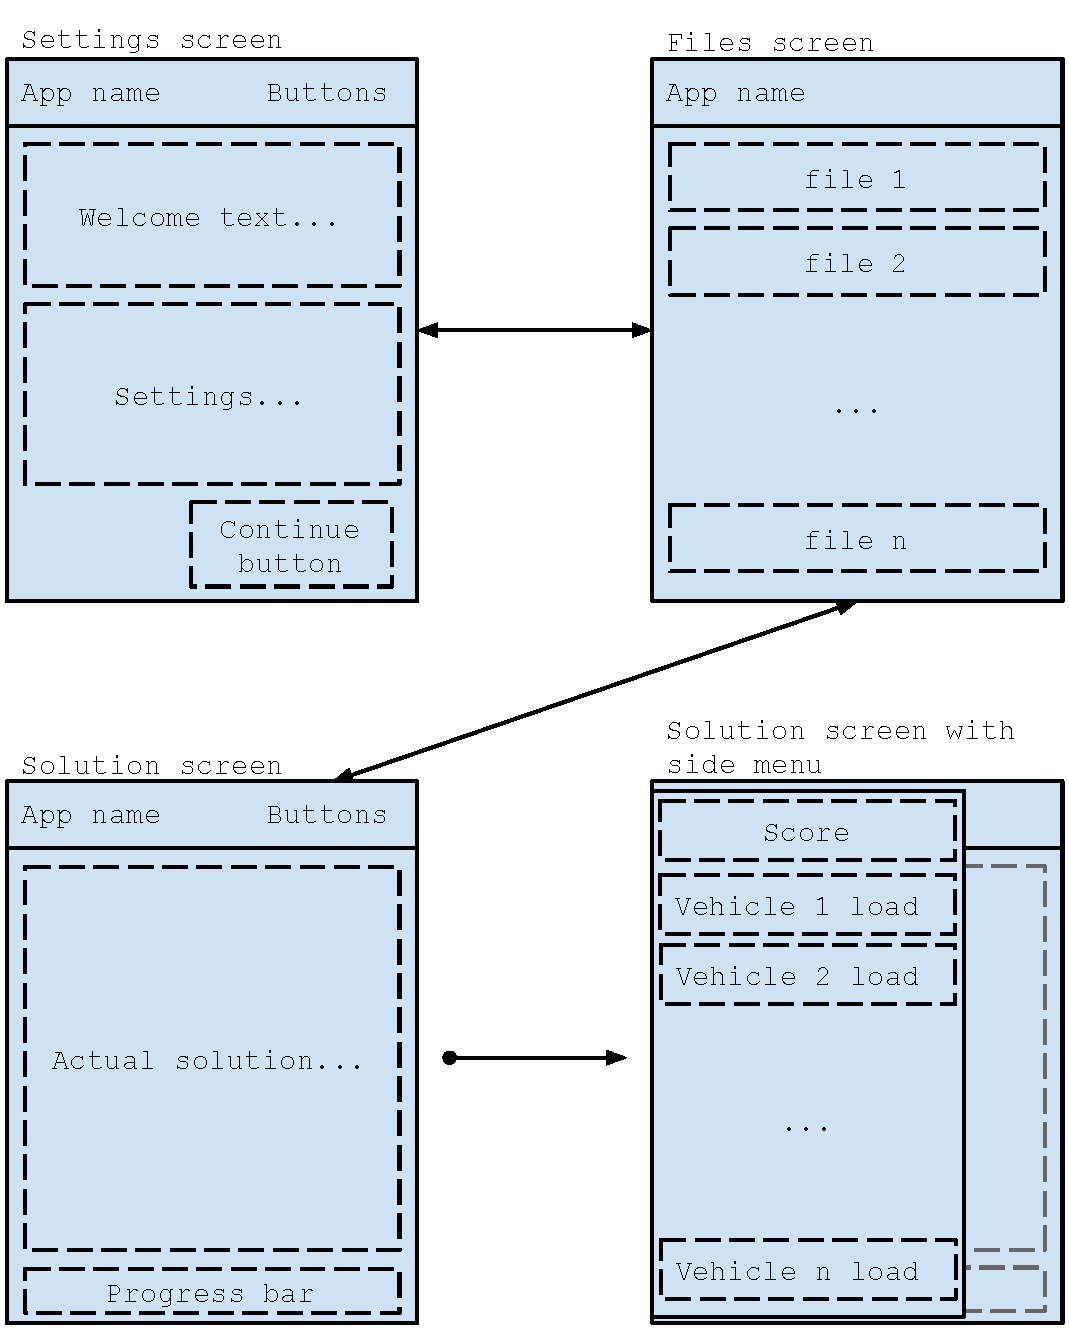
\includegraphics[scale=0.7]{fig/sceen_design.pdf}
    \caption{Design of screens and links among them.}
    \label{ScreenDesignFigure}
\end{figure}

\subsection{Design of screens}\label{ScreenDesignSection}
This section introduces design of application screens and describes component layouts. The overall concept and links
between screens are shown in Figure~\ref{ScreenDesignFigure}.

\paragraph{Application top bar}
Top bar is placed on the top of the each screen as shown in Figure~\ref{ScreenDesignFigure}. It contains name of the
application and quick function buttons. These buttons can start the calculation or call the informational dialogs.
Buttons are not visible all the time but only on the screens when it is necessary.

\paragraph{Settings screen}
The first screen of Figure~\ref{ScreenDesignFigure} is main screen of the application. It consists of top bar, welcome
text and part with setting elements where calculation options can be set. Last element on the screen is button for
switching to the next screen where one of the VRP files can be selected.

\paragraph{Screen with VRP files list}
The second screen in Figure~\ref{ScreenDesignFigure} contains only list of VRP files and top bar. Top bar does not
contains any buttons on this screen because there is no need for them. The list contains all of the included VRP files
and after click on one of them, it is switched to the last screen -- Solution screen.

\paragraph{Solution screen}
The most important screen of the application is the last screen. Solution and its gradual progress is displayed on this
screen. On the top bar, button for start of calculation is included and under the actual solution representation,
progress bar for displaying actual time is placed. When user swipe with finger from left to right on the screen, side
menu with actual solution statistic should be displayed.

\paragraph{Side menu with statistics}
The last section of Figure~\ref{ScreenDesignFigure} is side menu which is displayed on right side on the solution
screen. It contains statistic data of actual solution. First item on the menu is solution score and next items
represents every vehicle of the problem and its current load and capacity. Menu can be closed when user clicks somewhere
outside of the menu.

\paragraph{Informational dialogs}
Application design contains two informational dialogs for better understanding of the application content. First one
contains information about application itself. Second one consists of legend which describes all displayed components of
Vehicle Routing Problem on the screen.

\paragraph{Material design}
One of the new features which Android version 5 brings is material design. It is very sophisticated study that shows how
to handle elements, layouts, colors and others. Although this feature is not fully backward compatible, it is partially
possible to bring this design to earlier devices with older versions of Android. It is designed that application should
use material design as much as possible.

\section{Application implementation}\label{ApplicationImplementationSection}
In this section, implementation of Vehicle Routing Problem application is described. The first part introduces
application structure and its important components. Second part focuses on porting of Vehicle Routing Problem and its
model from the original OptaPlanner application. Graphical user interface is presented in the next
Section~\ref{GuiSection}.

\subsection{Application structure}
Application consists of one activity and three fragments as shown in Figure~\ref{ActivityFragmentsFigure}. Activity is
represented by \texttt{MainActivity} class in the application code and it contains Action bar and space where fragments
are placed. Every time when action of fragment change is invoked, the space is replaced by new fragment.

Settings elements are placed on the first fragment which is defined by \texttt{MainFragment} class.
\texttt{VrpFileListFragment} class represent the second fragment containing list of VRP files. The last fragment is
defined by \texttt{VrpFragment} class and it is used for displaying current solution.

\begin{figure}[h!]
    \centering
    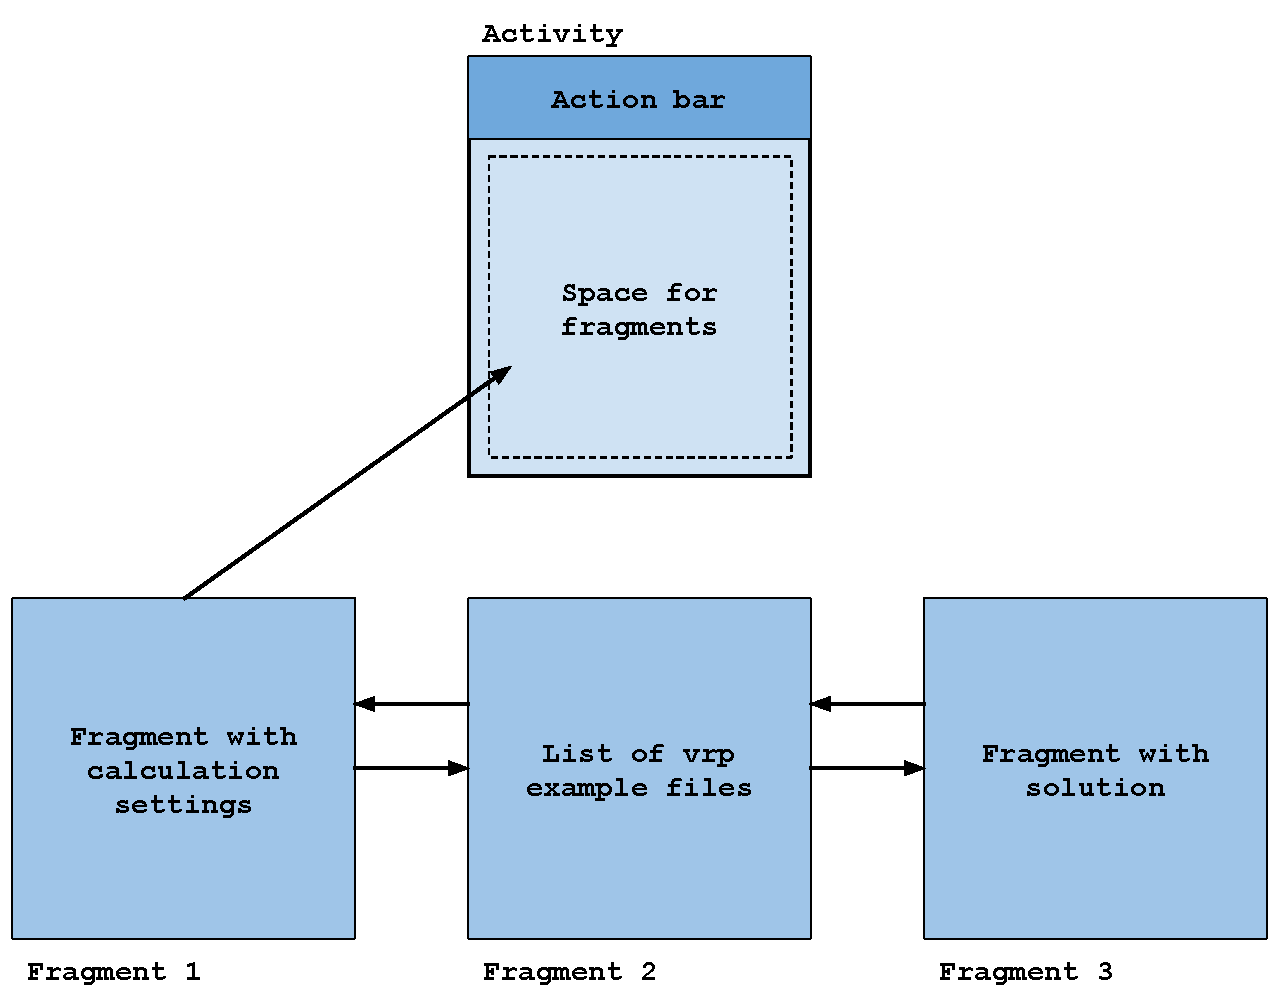
\includegraphics[scale=0.7]{fig/act_frag.pdf}
    \caption{Activity and fragments in application.}
    \label{ActivityFragmentsFigure}
\end{figure}

In the following paragraphs, important components of application are described. Especially, the components which are
related to the background processes. Graphical components and their layout are described in Section~\ref{GuiSection}.

\paragraph{List of files}
List of VRP example files is placed on the second fragment. This list is implemented by \texttt{RecyclerView} component
which simplifies displaying of data to the list and provides basic patterns of behavior.

\paragraph{Solver asynchronous process}
After the button for calculation start is pressed, asynchronous process is created. This process sets, builds and
activates Solver with required parameters. Listener is added to Solver to publish process every time when new best
solution is found. The process is represented by \texttt{VrpSolverTask} class which extends \texttt{AsyncTask}.
\texttt{AsyncTask} class enables changes of graphical user interface, perform the background operations and publishes
results.

\paragraph{Solution painter}
Solution painter is a~component which draws a~solutions on the screen. It is represented by \texttt{VrpPainter} class
which is modified \texttt{VehicleRoutingSolutionPainter} class from the original OptaPlanner project. Because Android
does not support Awt and Swing Java graphic libraries, \texttt{VehicleRoutingSolutionPainter} was rewritten to use
Android methods for drawing on the screen. Solution painter draws two types of solution:

\begin{enumerate}
    \item \textbf{Unsolved solution} --  painted when a~file is selected from the list in the second fragment.
    \item \textbf{New best solution} -- painted every time after Solver is activated and new best solution is found.
\end{enumerate}

\subsection{Porting of Vehicle Routing Problem}
Original Vehicle Routing application contains Vehicle Routing Problem model for OptaPlanner tool. These files are taken
and modified to fit in the created Android application. Following paragraphs present these files and show the way how
they are used.

\paragraph{Vehicle Routing Problem model}
Without model of the problem, application cannot work. Vehicle Routing Problem is defined by
\texttt{VehicleRoutingSolution} class which implements \texttt{Solution} interface. This class contains all information
about solved problem (list of all customers, depots and vehicles) and it is used together with solver configuration
by Solver to calculation of the problem. \texttt{Customer} class is marked as planned entity and contains
\texttt{Standstill} planning variable. More detailed information about Vehicle Routing Problem definition can be found
in OptaPlanner documentation~\cite{OptaPlannerDoc}.

\paragraph{Solver configurations}
In this application, it is possible to use three algorithms and set time limit of calculation. These configurations
include link to problem definition and link to score calculator and they are stored in \texttt{.xml} file which are used
for building the Solver. For each algorithm, there is one XML file and it is applied according to the choice in the
application. Time limit is additionally set after Solver is created.

\paragraph{Score calculator}
Every solution has its own score and this score must be calculated by one of the three methods described in
Section~\ref{ScoreConfigSection}. For score calculation in this application, \texttt{VehicleRoutingEasyScoreCalculator}
class which implements \texttt{EasyScoreCalculator} is used. This class calculates hard and soft score of solution. Hard
score is computed as a~load of vehicles above their capacity and soft score is calculated as neagative total vehicle
distance. In case of time window variant, delay against due time of arrival is added to the hard score.

\paragraph{VRP example files}
Example \texttt{.vrp} files are used as problem datasets. These files are taken from the original OptaPlanner Vehicle
Routing Problem application. They contain informations about number and capacity of vehicles, position and demands of
customers and position of depot. This application includes 36 example files in total.

\paragraph{Vehicle Routing importer}
Example files are stored in specific \texttt{.vrp} text format and have to be loaded into classes that describe Vehicle
Routing problem. For this purpose, \texttt{VehicleRoutingImporter} class is imported and used from the original
OptaPlanner application.

\section{Graphical user interface}\label{GuiSection}
This section presents graphical user interface implementation of the application as designed in
Section~\ref{ScreenDesignSection}. The first part of this section describes application screens and the second part
introduces three important components.

\subsection{Application screens}
Every application consists of Fragments or Activities which are collectively called screens. Using controls, it is
possible to move from one screen to another or to change its appearance or behavior. This application is composed from
three screens. These screens can be seen in Figure~\ref{ApplicationScreensFigure}. The third screen is displayed with
unsolved problem and with ongoing solution process.

\paragraph{Main screen}
Main screen is displayed after the application starts. It consists from Action bar, welcome text, setting elements
and button to continue to another screen. Action bar contains application name and buttons for displaying legend dialog
and application information dialog. Welcome text provides some basic instruction for the users. Two controls are present
for calculation options of the problem. It is possible to set time limit in seconds using Number picker and Spinner
allows to select one of the three supported algorithms. Last element on this screen is Open file button which opens
screen with list of VRP files.

\paragraph{Screen with VRP files list} After Open file button on the main screen is pressed, screen with VRP files is
displayed. It also contains action bar but it is very limited because no controls are required on this screen. Rest of
area is filled with list of VRP files from original OptaPlanner application~\cite{OptaPlannerDistribution}. After the
selected file is pressed, it is switched to last screen and the problem with its solutions is displayed.

\paragraph{Solution screen}
This screen is used to display unsolved, ongoing and solved solutions. It contains Action bar with all of the control
items as shown in Figure~\ref{ApplicationScreensFigure}. Compared to the main screen, Action bar has an~additionally
button for displaying Navigation drawer and button for start and end of the solution process. On the bottom of the
screen, Progress bar is placed. This component is used for displaying time which approximately remains. Rest of the
screen is filled with component which draws current solution. At the beginning, the component draws unsolved solution
and after the start button is pressed, it always draws the best solution after it is found. Individual elements of this
component are:

\begin{itemize}
  \item \textbf{Circle with a~number} -- customer with his demand.
  \item \textbf{Building image} -- depot from where vehicles depart.
  \item \textbf{Car image} -- vehicle with its color.
  \item \textbf{Solid line} -- vehicle road to a~customer.
  \item \textbf{Dashed line} -- vehicle road to a~depot.
  \item \textbf{Sector on a~circle} -- time windows for vehicle arrival.
  \item \textbf{Line on a~circle} -- vehicle arrival time.
\end{itemize}

\begin{figure}[h!]
    \centering
    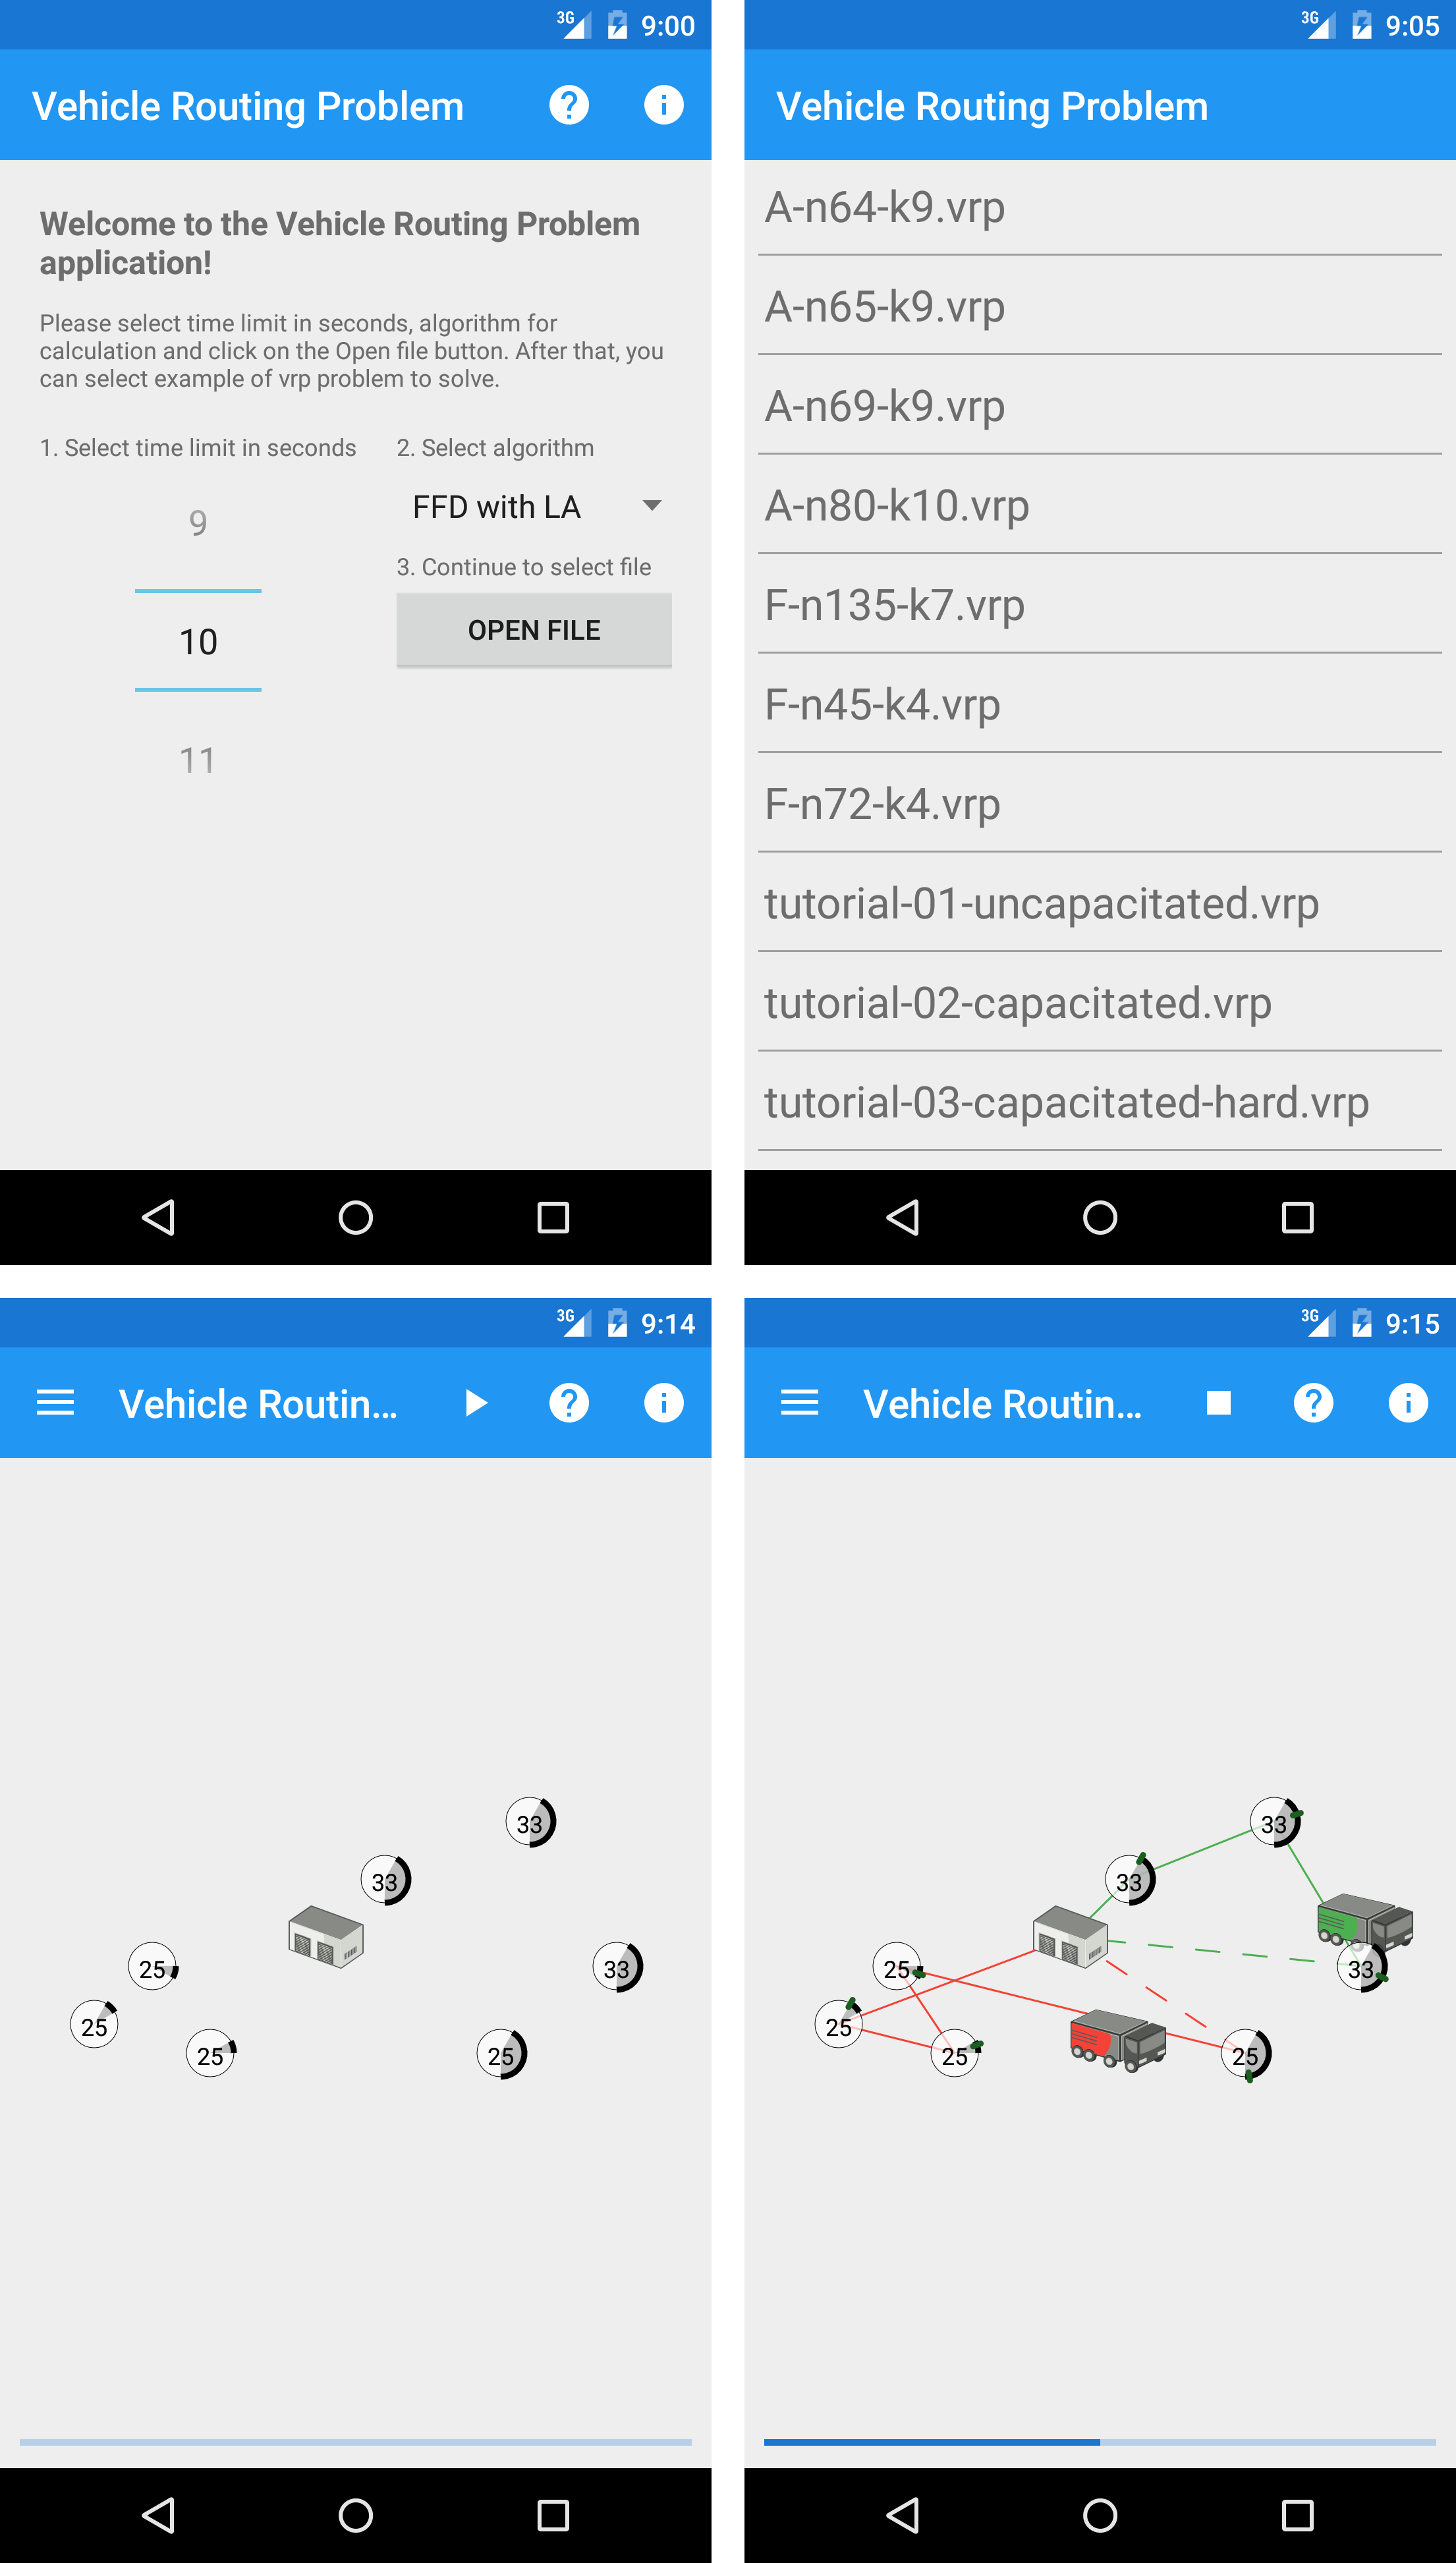
\includegraphics[scale=0.15]{fig/screens.png}
    \caption{Application screens -- main screen, list of VRP files, screen with unsolved problem and ongoing solution
    process.}
    \label{ApplicationScreensFigure}
\end{figure}

\subsection{Application components}
This section introduces and describes three important components of the application: Action bar, Navigation drawer and
Dialogs.

\subsubsection{Action bar}
Action bar is a~panel on top of the screen that provides basic user action and informations about user navigation. It
always contains application name, optionally action buttons for quick invocation of application functionality and
overflow button on the right side for displaying the other applications options.

Action bar is displayed on every screen of this application but it changes depending on required functions on actual
screen. Figure~\ref{ApplicationScreensFigure} shows action bars of each screen.

\subsubsection{Navigation drawer}
Navigation drawer is a~panel that displays application navigation on the left edge of the screen. By default, it is
hidden and it could be displayed by touching the left icon on the action bar. Also, it could be displayed when a~user
swipes with a~finger from the left edge of the screen to the right. Opposite procedure makes navigation drawer
invisible.

This application uses navigation drawer for displaying important statistic data. Figure~\ref{NavigationDrawerFigure}
displays visible panel on the left side of the application. The first item on the panel shows hard and soft score of
displayed solution. Second item holds total distance traveled. Other items are linked to vehicles of the problem. Each
of them has its own parameters -- color, name and capacity. These three items are static and do not change during the
calculation. Last parametr is actual load of the vehicle.
\\
\begin{figure}[h!]
    \centering
    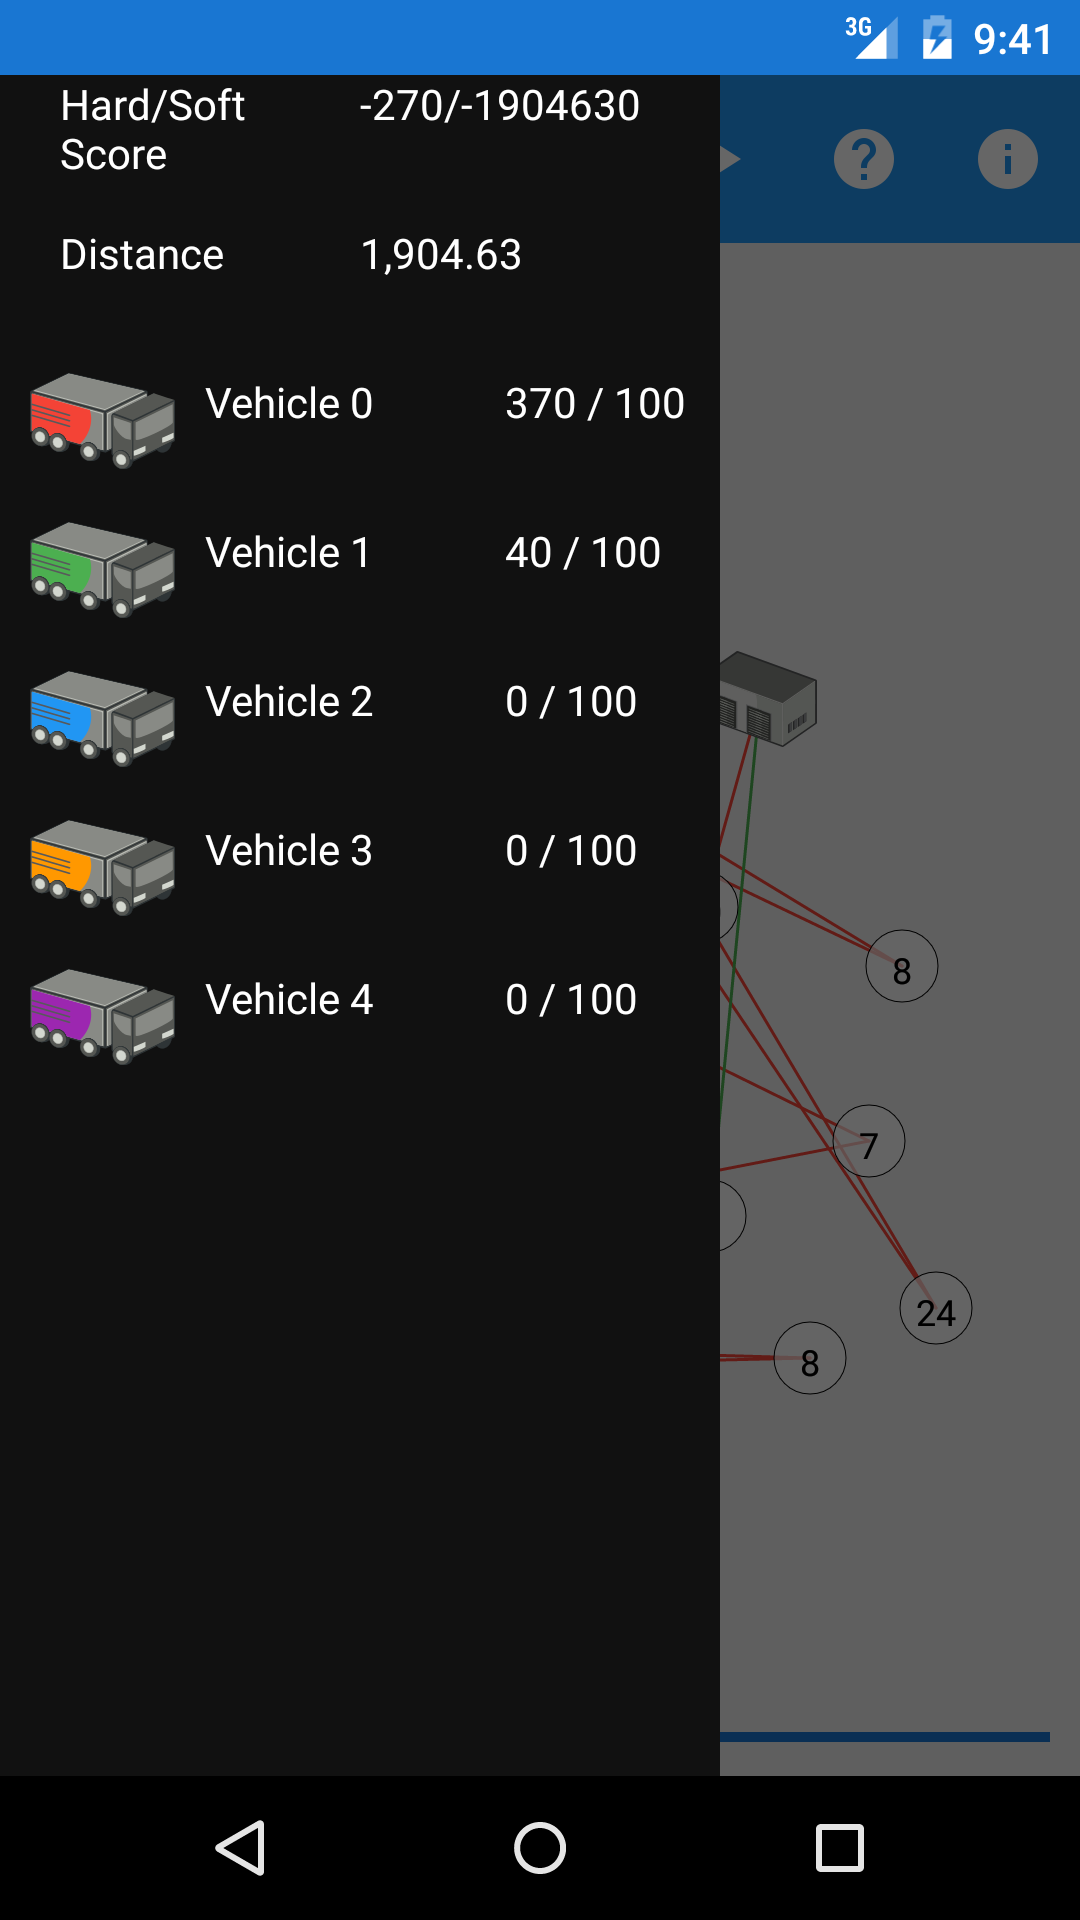
\includegraphics[scale=0.15]{fig/nav_drawer.png}
    \caption{Navigation drawer with actual data.}
    \label{NavigationDrawerFigure}
\end{figure}

\subsubsection{Dialogs}
Dialogs are small windows which display some significant informations or they are used for user interaction with
decisions that define further actions. Dialogs are always located above all other parts of the application.

Figure~\ref{DialogsFigure} shows all three dialogs used in the application. The first one and the second one can be
retrieved directly from the action bar by clicking on the icons with question mark or informative icon. The first dialog
contains application legend for understanding what is displayed on the screen and the second dialog briefly describes
the application. The last dialog is displayed only when calculation runs and user clicks on the back button. Dialog then
asks the user if he wants to end the ongoing calculation.
\\
\begin{figure}[h!]
    \centering
    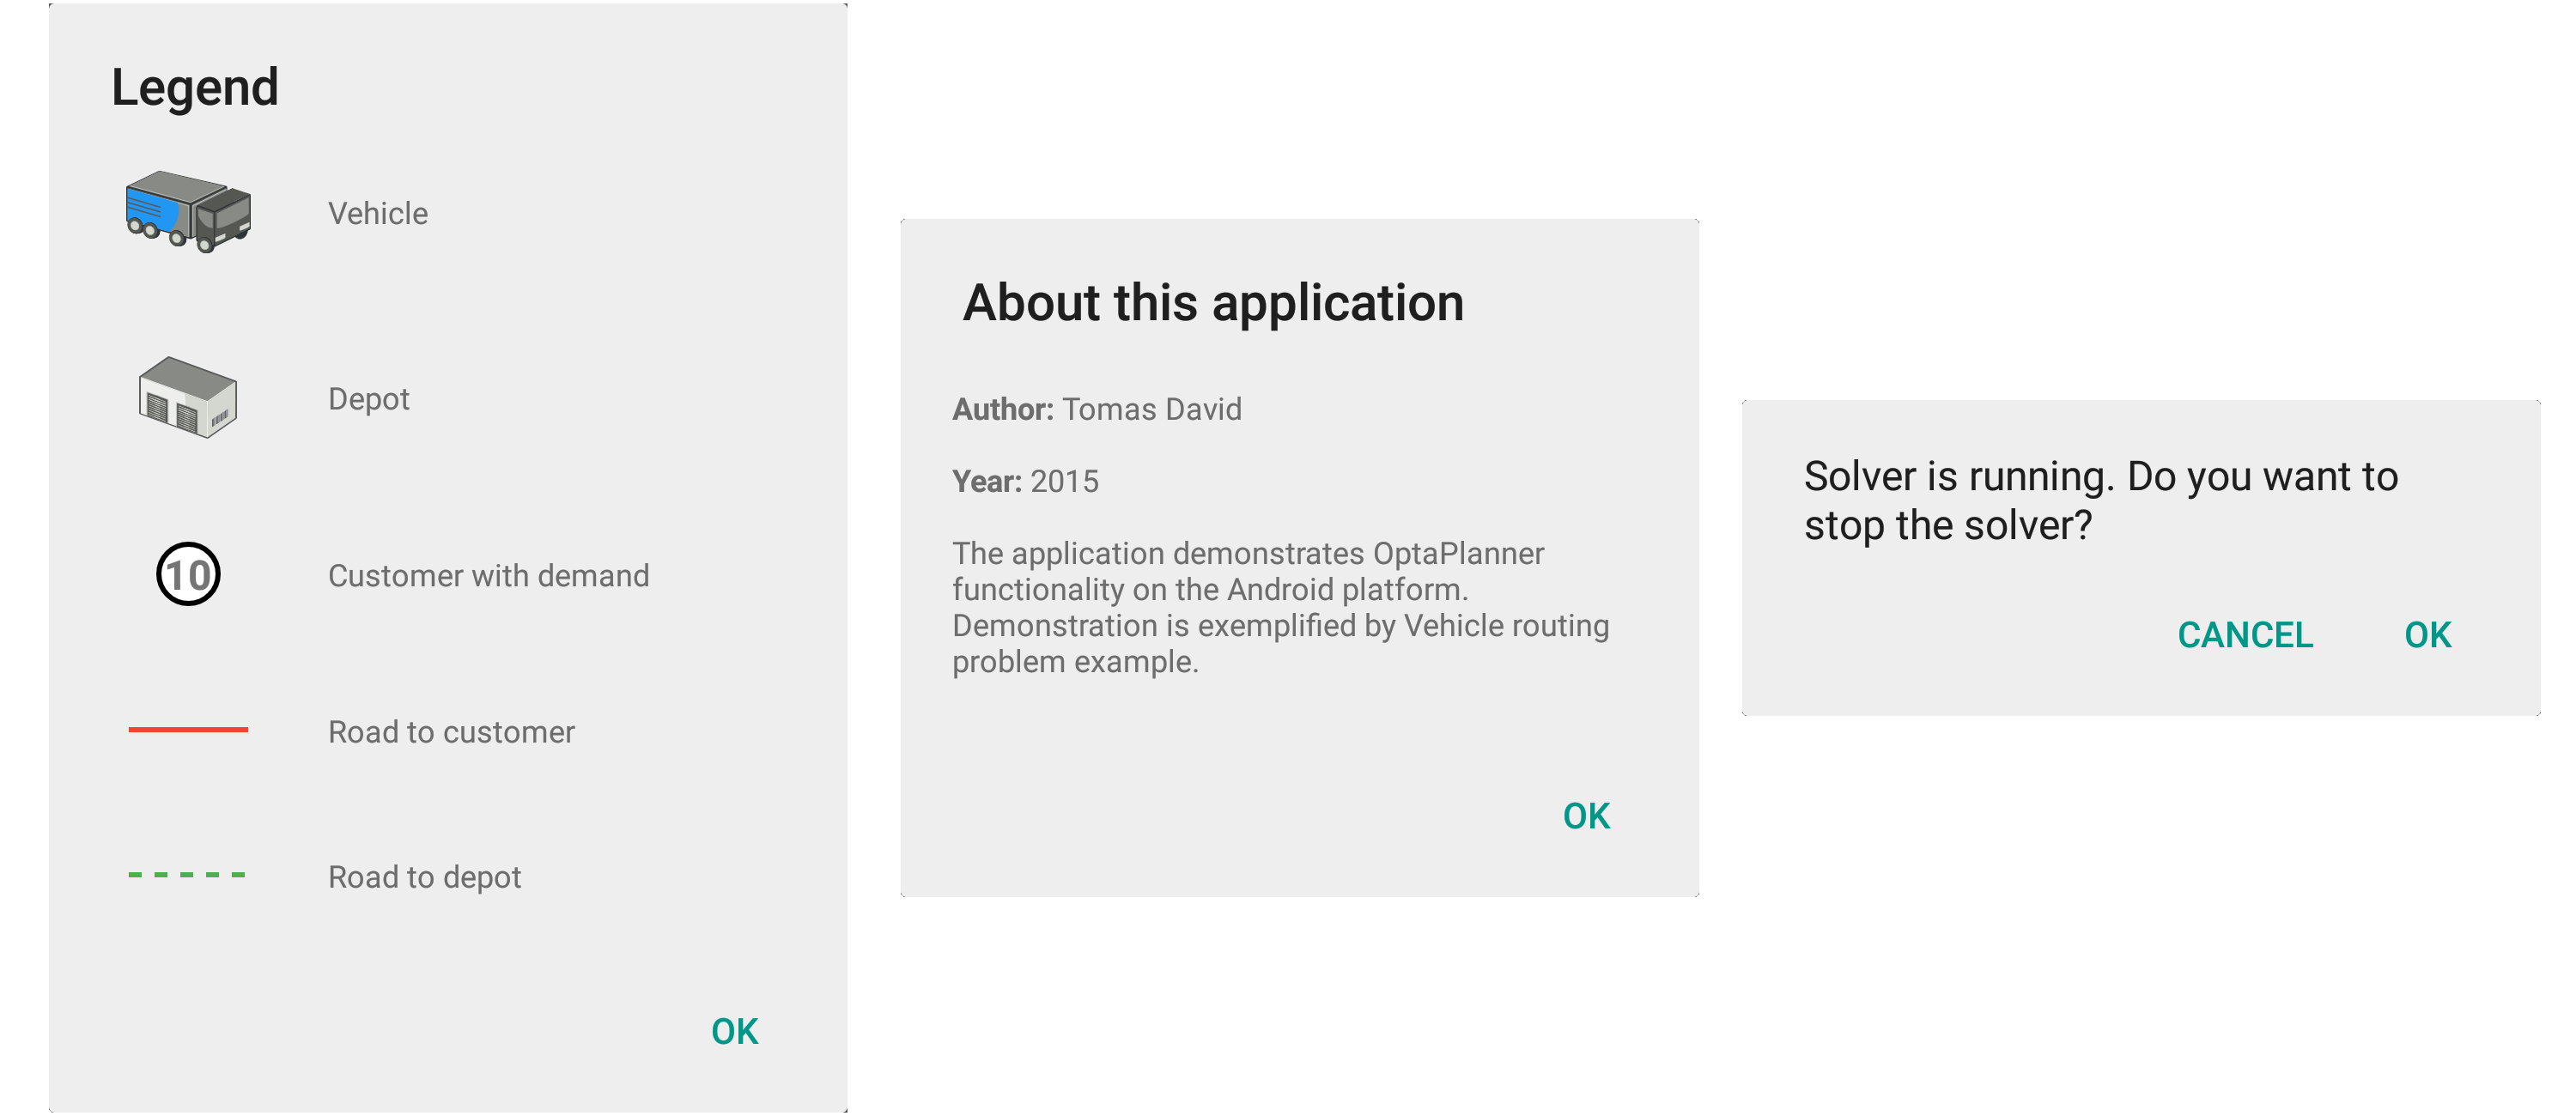
\includegraphics[scale=0.15]{fig/dialogs.png}
    \caption{Screenshots of dialogs used in the application.}
    \label{DialogsFigure}
\end{figure}
